\documentclass[Main.tex]{subfiles}
\begin{document}
\section{Outlier detection}
Additionally, there is no clear guidance in any of the Bland-Altman papers on the treatment of outliers that may arise in a plot. Bland and Altman attend to the issue of outliers in their 1986
paper, wherein they present a data set with an extreme outlier.
An example used in Bland-Altman 1986 identifies a “clear outlier”, where it is advised by the authors that “in practice, one could omit this subject”.
Bland and Altman 1999 recommend the computationally intensive approach of calculating the limits of agreement with, and then without, suspected outliers, in order to assess the impact on the results. However, they are clear that they do not recommend excluding outliers from analyses.


\section{Outliers}

The Bland-Altman plot also can be used to identify outliers. An
outlier is an observation that is conspicuously different from the
rest of the data that it arouses suspicion that it occurs due to a
mechanism, or conditions, different to that of the rest of the
observations. Classification of outliers can be determined with
numerous established approaches, such as the Grubb's test, but
always classification must be informed by the logic of the data's
formulation. Figure 1.6 is a Bland-Altman plot with two potential
outliers.


\citet*{BA99} do not recommend excluding outliers from analyses,
but remark that recalculation of the inter-method bias estimate,
and further calculations based upon that estimate, are useful for
assessing the influence of outliers. The authors remark that `we
usually find that this method of analysis is not too sensitive to
one or two large outlying differences'.

Figure 1.6 demonstrates how the Bland-Altman
plot can be used to visually inspect the presence of potential
outliers.

\subsection{Bartko's Ellipse}
As a complement to the Bland-Altman plot, \citet{Bartko} proposes
the use of a bivariate confidence ellipse, constructed for a
predetermined level. \citet{AltmanEllipse} provides the relevant calculations for the ellipse. This ellipse is intended as a visual
guidelines for the scatter plot, for detecting outliers and to
assess the within- and between-subject variances.


Bartko states that the ellipse can, inter alia, be
	used to detect the presence of outliers (furthermore
	\citet{Bartko} proposes formal testing procedures, that shall be
	discussed in due course). Inspection of Figure 1.7 shows that the
	fourth observation is outside the bounds of the ellipse,
	concurring with the conclusion that it is an outlier.


The minor axis relates to the between subject variability, whereas
the major axis relates to the error mean square, with the ellipse
depicting the size of both relative to each other.
Consequently Bartko's ellipse provides a visual aid to determining the
relationship between variances. If $\mbox{var}(a)$ is greater than $\mbox{var}(d)$, the orientation of the ellipse is horizontal. Conversely if $\mbox{var}(a)$ is less than $\mbox{var}(d)$, the orientation of the ellipse is vertical.


%(Furthermore \citet{Bartko}
%proposes formal testing procedures, that shall be discussed in due
%course.)

The Bland-Altman plot for the Grubbs data, complemented by Bartko's ellipse, is depicted in Figure 1.7.
The fourth observation is shown to be outside the bounds of the ellipse, indicating that it is a potential outlier.


\begin{figure}[h!]
	% Requires \usepackage{graphicx}
	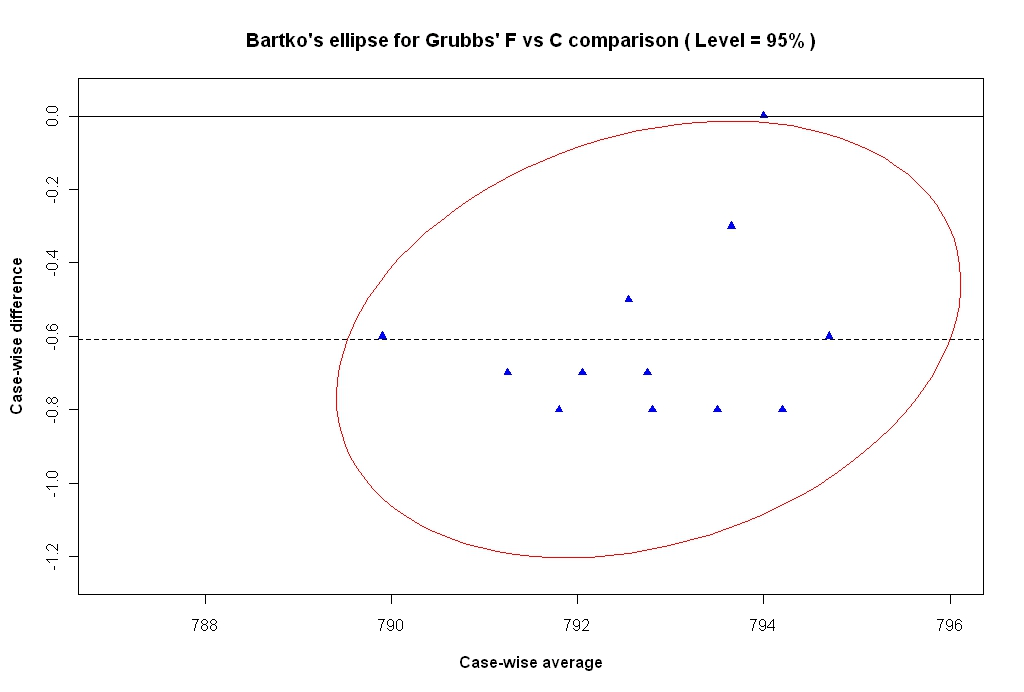
\includegraphics[width=130mm]{images/GrubbsBartko.jpeg}
	\caption{Bartko's Ellipse For Grubbs' Data.}\label{GrubbsBartko}
\end{figure}

The limitations of using bivariate approaches to outlier detection
in the Bland-Altman plot can demonstrated using Bartko's ellipse.
A covariate is added to the `F vs C' comparison that has a
difference value equal to the inter-method bias, and an average
value that markedly deviates from the rest of the average values
in the comparison, i.e. 786. 

	
Table 1.8 depicts a $95\%$ confidence
ellipse for this manipulated data set. By inspection of the
confidence interval, a conclusion would be reached that this extra
covariate is an outlier, in spite of the fact that this
observation is wholly consistent with the conclusion of the
Bland-Altman plot.
	

	
\begin{figure}[h!]
	% Requires \usepackage{graphicx}
	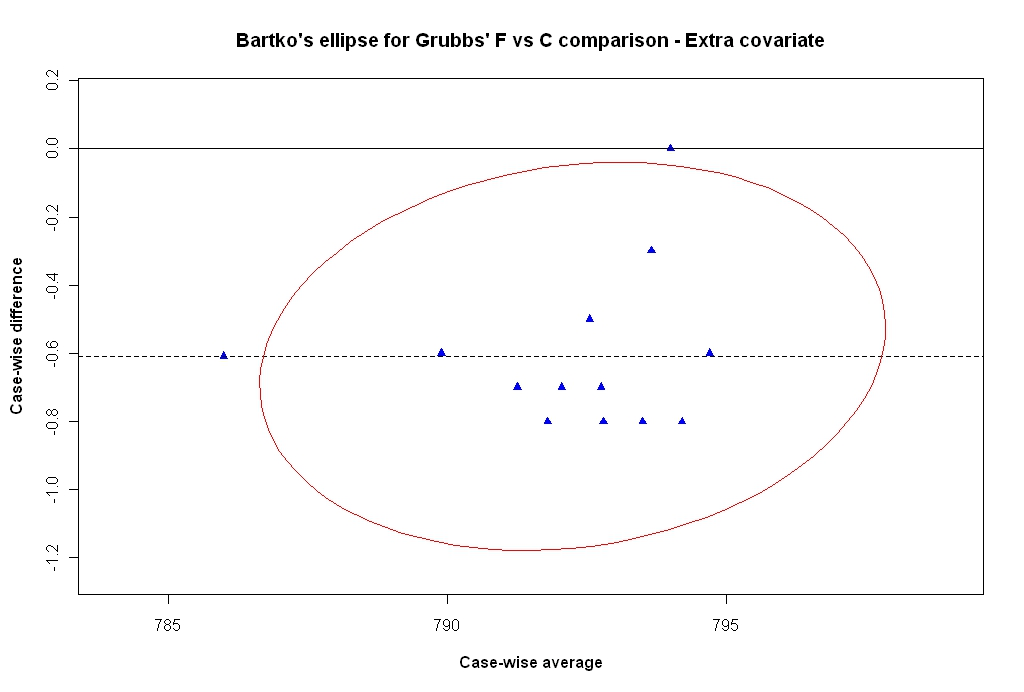
\includegraphics[width=130mm]{images/GrubbsBartko2.jpeg}
	\caption{Bartko's Ellipse For Grubbs' Data, with an extra covariate.}\label{GrubbsBartko2}
\end{figure}


Importantly, outlier classification must be informed by the logic of the
data's formulation. In the Bland-Altman plot, the horizontal displacement of any
observation is supported by two independent measurements. Any
observation should not be considered an outlier on the basis of a
noticeable horizontal displacement from the main cluster, as in
the case with the extra covariate. Conversely, the fourth
observation, from the original data set, should be considered an
outlier, as it has a noticeable vertical displacement from the
rest of the observations.

%Grubbs' test is a statistical test used for detecting outliers in a
%univariate data set that is assumed to be normally distributed.

%\citet{Grubbs} defined an outlier as a co-variate that appears to
%deviate markedly from other members of the sample in which it
%occurs.

	
In the Bland-Altman plot, the horizontal displacement of any
	observation is supported by two independent measurements. Any
	observation should not be considered an outlier on the basis of a
	noticeable horizontal displacement from the main cluster, as in
	the case with the extra co-variate. Conversely, the fourth
	observation, from the original data set, should be considered an
	outlier, as it has a noticeable vertical displacement from the
	rest of the observations.
	
	Bartko's ellipse provides a visual aid to determining the
	relationship between variances. If $\mbox{var}(a_{i})$ is greater
	than $\mbox{var}(d_{i})$, the orientation of the ellipse is
	horizontal. Conversely if $\mbox{var}(a_{i})$ is less than
	$\mbox{var}(d_{i})$, the orientation of the ellipse is vertical.
	\newpage


\subsection{The Grubbs Test}
In classifying whether a observation from a univariate data set is
an outlier, many formal tests are available, such as the Grubbs test for outliers. In assessing
whether a covariate in a Bland-Altman plot is an outlier, this
test is useful when applied to the case-wise difference values treated as a
univariate data set. The null hypothesis of the Grubbs test procedure is the absence
of any outliers in the data set. Conversely, the alternative hypotheses is that there is at least one outlier
present.

	%\citet{Grubbs} defined an outlier as a co-variate that appears to
	%deviate markedly from other members of the sample in which it
	%occurs.
	
	In classifying whether a observation from a univariate data set is
	an outlier, Grubbs' outlier test is widely used. In assessing
	whether a co-variate in a Bland-Altman plot is an outlier, this
	test is useful when applied to the difference values treated as a
	univariate data set. For Grubbs' data, this outlier test is
	carried out on the differences, yielding the following results.
	
	The null and alternative hypotheses is the absence and presence of
	at least one outlier respectively. Grubbs' outlier test statistic
	$G$ is the largest absolute deviation from the sample mean divided
	by the standard deviation of the differences. 
	
	
The test statistic for the Grubbs test ($G$) is the largest
absolute deviation from the sample mean divided by the standard
deviation of the differences,
\[
G =  \displaystyle\max_{i=1,\ldots, n}\frac{\left \vert d_i -
	\bar{d}\right\vert}{S_{d}}.
\]

For the `F vs C' comparison it is the fourth observation gives
rise to the test statistic, $G = 3.64$. The critical value is
calculated using Student's $t$ distribution and the sample size,
\[
U = \frac{n-1}{\sqrt{n}} \sqrt{\frac{t_{\alpha/(2n),n-2}^2}{n - 2
		+ t_{\alpha/(2n),n-2}^2}}.
\]
For this test $U = 0.75$. The conclusion of this test is that the fourth observation in the `F vs C' comparison is an outlier, with $p-$value = 0.003, according with the previous result using Bartko's ellipse.


	
	

	
	For the `F vs C'
	comparison, $G = 3.6403$. The critical value is calculated using
	Student's $t$ distribution and the sample size,
	\begin{equation}
	U = \frac{n-1}{\sqrt{n}} \sqrt{\frac{t_{\alpha/(2n),n-2}^2}{n - 2
			+ t_{\alpha/(2n),n-2}^2}}.
	\end{equation}
	
	For this test $U = 0.7501$. The conclusion of this test is that
	the fourth observation in the `F vs C' comparison is an outlier,
	with $p-value = 0.002799$.
	

	
	
	%\begin{figure}[h!]
	%\begin{center}
	%  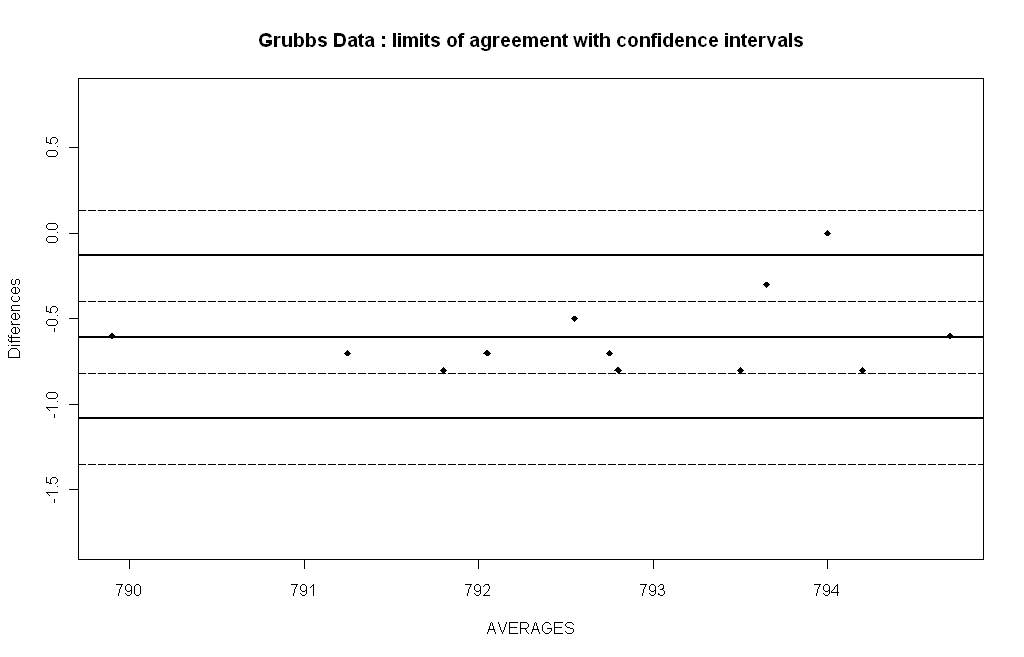
\includegraphics[width=125mm]{images/GrubbsLOAwCIs.jpeg}
	%  \caption{Limits of agreement with confidence intervals}\label{LOAwCIs}
	%\end{center}
	%\end{figure}









\section{Treatment of Outliers}



	\subsection{Effect of Outliers} Another argument against
	the use of model I regression is based on outliers. Outliers can
	adversely influence the fitting of a regression model. Cornbleet
	and Cochrane compare a regression model influenced by an outlier
	with a model for the same data set, with the outlier excluded from
	the data set. A demonstration of the effect of outliers was made
	in Bland Altman's 1986 paper. However they discourage the
	exclusion of outliers.
	
	\section{Indications on how to deal with outliers in Bland Altman plots}
	
	We wish to determine how outliers should be treated in a Bland
	Altman Plot
	
	In their 1983 paper they merely state that the plot can be used to
	'spot outliers'.
	
	In  their 1986 paper, Bland and Altman give an example of an
	outlier. They state that it could be omitted in practice, but make
	no further comments on the matter.

\subsection*{Bland Altman 1999}
	In Bland and Altmans 1999 paper, we get the clearest indication of
	what Bland and Altman suggest on how to react to the presence of
	outliers. Their recommendation is to recalculate the limits
	without them, in order to test the difference with the calculation
	where outliers are retained.\\
	
	The span has reduced from 77 to 59 mmHg, a noticeable but not
	particularly large reduction.
	\\
	However, they do not recommend removing outliers. Furthermore,
	they say:
	\\
	We usually find that this method of analysis is not too sensitive
	to one or two large outlying differences.
	\\
	We ask if this would be so in all cases. Given that the limits of
	agreement may or may not be disregarded, depending on their
	perceived suitability, we examine whether it would possible that
	the deletion of an outlier may lead to a calculation of limits of
	agreement that are usable in all cases?
	\\
	Should an Outlying Observation be omitted from a data set? In
	general, this is not considered prudent.
	\\
	Also, it may be required that the outliers are worthy of
	particular attention themselves.
	\\
	Classifying outliers and recalculating We opted to examine this
	matter in more detail. The following points have to be considered
	\\how to suitably identify an outlier (in a generalized sense)
	\\Would a recalculation of the limits of agreement generally
	results in  a compacted range between the upper and lower limits
	of agreement?
	%=====================================================================%	
	\addcontentsline{toc}{section}{Bibliography}
	\bibliography{2017bib}	
\end{document}
